\section{Introduction}

One class classification (OCC) is an instance of binary classification where all the points of the dataset at hand belong to the same (positive) class. The challenge of this task is to construct a decision boundary without using points from the other (negative) class. It has various safety-critical applications in anomaly detection, for instance to detect banking fraud, cyber-intrusion or industrial defect, in out-of-distribution detection, to prevent wrong decisions of Machine Learning models, or in Open-Set-Recognition. However, OCC algorithms suffer from limitations such as the \textbf{lack of negative data}, and \textbf{robustness issues} \cite{occrobust}, the latter being an under-explored topic in the OCC spectrum. Even though some algorithms do not use negative examples, many work cope with the lack of negative data with Negative Sampling, either artificially \cite{sipple_interpretable_2020} or using outlier exposure \cite{hendrycks_benchmarking_2019,fort_exploring_2021}. However, such samplings are often biased or heuristic. As for robustness, although some works design robust algorithms \cite{goyal_drocc_2020,lo_adversarially_2022}, it is always only empirically demonstrated \cite{hendrycks_benchmarking_2019}. 

\begin{figure*}[!t]
    \centering
    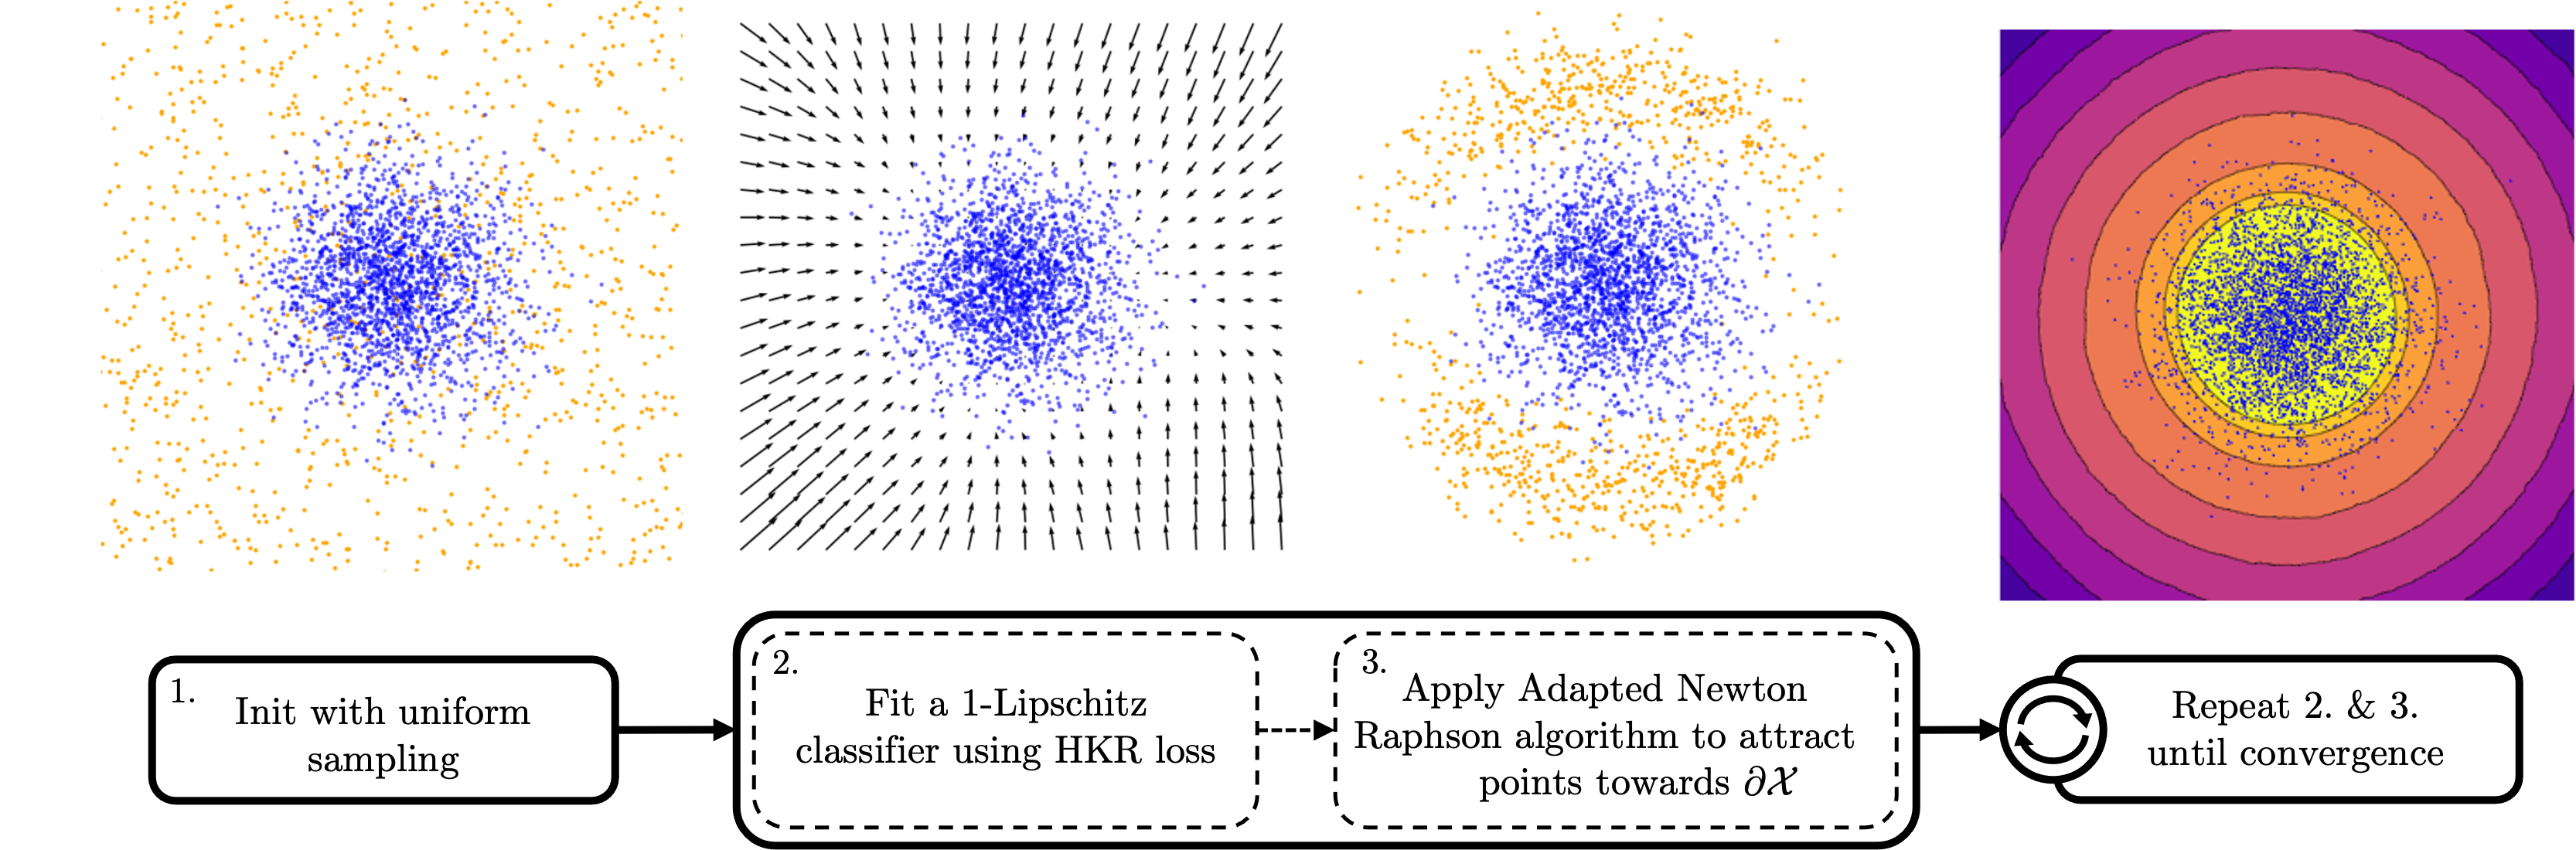
\includegraphics[width=0.9\linewidth, trim=0 0 0 0, clip]{images/mainfigure.png}
    \caption{Summary of One Class Signed Distance Function (OCSDF). We start with an uniform negative sampling, then we fit a 1-Lipschitz classifier $f_{\theta}$ using the Hinge Kantorovich-Rubinstein loss. We apply the Adapted Newton Raphson algorithm \ref{alg:newtonraphson} to attract the points towards the boundary of the domain $\partial \mathcal{X}$ thanks to the smoothness of $f_{\theta}$, which in addition allows providing robustness certificates.}
    \label{fig:main}
    %\vspace{-0.3cm}
\end{figure*}


In this paper, we introduce a new framework to perform OCC based on the Signed Distance Function (SDF), a function traditionally used in computer graphics. Assume the positive samples are independently and identically obtained from a distribution $\Prob_X$ with compact support $\support\subset\Reals^d$. Let $\partial\support=\closure{\support}/\interior{\support}$ be the boundary of the distribution. The Signed Distance Function is the function $\Sdf:\Reals^d\rightarrow\Reals$:
\begin{equation}
\Sdf(x)=\begin{cases}
d(x,\partial\support)&\text{ if }x\in\support,\\
-d(x,\partial\support)&\text{ otherwise,}\\
\end{cases}
\end{equation}
where $d(x,\partial\support)=\inf_{z\in\partial\support} \|x-z\|_2$. The idea of our algorithm, which we call One Class Signed Distance Function (OCSDF) is to learn the SDF to the boundary of the positive data distribution and use it as a normality score. We show that the Hinge Kantorovich-Rubinstein (HKR) loss introduced by~\cite{serrurier2021achieving} allows provably learning the SDF with a 1-Lipschitz network. 

SDF exhibits desirable properties. First, by implicitly parametrizing the domain $\support$, it allows efficiently sampling points outside of $\support$ and performing principled Negative Sampling. Second, the SDF fulfils the Eikonal equation: $\|\nabla_x \Sdf(x)\|=1$. In particular, $\Sdf$ is 1-Lipschitz with respect to $l2$-nom : $\forall x,z\in\Reals^d, \|\Sdf(x)-\Sdf(z)\|_2\leq \|x-z\|_2$. This property provides exact robustness certificates for OCSDF in the form of a certified AUROC that can be computed at the same cost as AUROC. This regularity translates into solid empirical robustness as compared to other OCC baselines. In other words, OCSDF alleviates the \textbf{lack of negative data} and the \textbf{robustness issue}. We go further and highlight interesting research perspectives regarding OCSDF. Indeed, we show that learning the SDF with a 1-Lipschitz network enables a generative procedure that allows visualizing points at the boundary of $\support$. Moreover, It implicitly parametrizes the shape of $\support$, which connects One-Class Classification with implicit surface parametrization, intensively used in computer graphics for shape reconstruction. 

Our contributions are as follows. \textbf{(1)} We introduce a new OCC framework based on the Signed Distance Function to the boundary of the data distribution. We theoretically demonstrate that the SDF can be learned with a 1-Lipschitz neural net using the Hinge Kantorovich-Rubinstein (HKR) loss and Negative Sampling; \textbf{(2)} We evaluate the performances of OCSDF on several benchmarks and show its benefits for theoretical and empirical robustness; and \textbf{(3)} we demonstrate how OCSDF extends the applications of One Class Classification from traditional OOD detection to generative visualization and implicit surface parametrization for shape reconstruction from point clouds.


% \begin{enumerate}
%     \item We propose to parametrize ground truth $\Sdf$ with a 1-Lipschitz neural net thanks to Property~\ref{thm:sdf1lip}. The model is \textit{robust by design} thanks to the robustness certificates provided by 1-Lipschitz architectures. This gives formal guarantees against adversarial attacks, and allows to use the SDF in raymarching algorithms with correctness guarantees.   
%     \item Then, we show that the Hinge Kantorovich-Rubinstein (HKR) loss introduced by~\cite{serrurier2021achieving} allows to provably learn the SDF with a 1-Lipschitz network. This does not requires access to ground truth signed distance, unlike approaches based on least squares minimization. This allows to extend the use of SDF to high dimensional datasets (e.g images), not only 2D/3D like done ordinarily.
%     \item We illustrate the soundness of our approach on three benchmarks: supervised One Class learning on images data, unsupervised Anomaly Detection on tabular data, and Neural Implicit Surface learning from 3D point clouds.
% \end{enumerate}

% Finally, the link of HKR loss with optimal transport yields meaningful interpretations of the saliency maps of the model, in a fashion that reminds diffusion models.



%\vspace{-0.1cm}
\section{Related Work}

\paragraph{One Class Classification (OCC)} OCC is an instance of binary classification where all the points of the dataset at hand belong to the same (positive) class. The challenge of this task is to construct a decision boundary without using points from the other (negative) class. OCC amounts to finding a domain containing the support of the data distribution. That is why OCC is mainly used in Out Of Distribution (OOD), anomaly or novelty detection, with positive samples considered In Distribution (ID) and negative ones as OOD, anomalies or novelties. This task dates back to \cite{sager_iterative_1979, hartigan_estimation_1987} and was popularized for anomaly detection with One-class Support Vector Machines (OC-SVM)\cite{scholkopf_support_1999}. Since then, the field of OCC has flourished with many well-established algorithms such as Local Outlier Factors \cite{breuning_lof_2000}, Isolation Forests \cite{liu2008isolation} and their variants (see \cite{han_adbench_nodate} for a thorough benchmark). More recently, since Deep-SVDD \cite{ruff2018deep} - followed by several works such as \cite{bergman2019classification,golan_geometric_2018,goyal_drocc_2020,zenati_adversarially_2018,sabokrou2018adversarially} - Deep Learning has emerged as a relevant alternative to perform OCC due to its capacities to handle large dimensional data. However, methods of this field suffer from their lack of \textbf{robustness and certifications}, which makes them vulnerable to adversarial attacks. In addition, they always struggle to cope with the \textbf{lack of OOD data}. In this paper, we tackle these problems with an OCC algorithm based on approximating the SDF using \textbf{1-Lipschitz neural nets}. In addition, the SDF being intensively used in Computer Graphics, our algorithm establishes a new link between OCC and \textbf{implicit surface} parametrization.

%\vspace{-0.1cm}
\paragraph{SDF for neural implicit surfaces}

Historically, signed distance functions have been used in computer graphics to parametrize a surface as the level set of some function~\cite{novelloExploringDifferentialGeometry2022}. Given an incomplete or unstructured representation of a geometrical object (like a 3D point cloud or a triangle soup), recent methods aim at representing a smooth shape either as vectors in the latent space of a generative model~\cite{achlioptasLearningRepresentationsGenerative2018, ben-hamuMultichartGenerativeSurface2018, groueixAtlasNetPapierMAch2018, chouGenSDFTwoStageLearning2022} or directly as parameters of a neural net~\cite{parkDeepSDFLearningContinuous2019, atzmonSALSignAgnostic2020}.
The first method allows for easy shape interpolation, while the latter proved to be a more robust approach~\cite{daviesEffectivenessWeightEncodedNeural2021}. Those neural implicit surfaces alleviate both the problems related to memory requirements of voxel-based representations and the combinatorial nature of meshes, making them ideally suited for rendering using ray marching~\cite{hartSphereTracingGeometric1995} and constructive solid geometry. In those contexts, the constraint $\|\nabla_x f(x)\|\leq 1$ is necessary to guarantee the validity of the geometrical query while having $\|\nabla_x f(x)\|$ as close as possible to 1 allows for greedier queries and faster computation times. In practice, training an SDF requires a dataset $(p,d)$ of points $p \in \mathbb{R}^3$ with their corresponding signed distance $d$ to the desired surface. Computing those distances requires the existence and availability of a ground truth, which is not always the case. Moreover, training tends to be unstable in general, and special care is needed for most computer graphics applications~\cite{sharpSpelunkingDeepGuaranteed2022}. Our method can instead be trained to approximate a surface without prior knowledge of the distances and is provably robust.

%\vspace{-0.15cm}
\paragraph{1-Lipschitz neural nets}

As noticed in~\cite{bethune2022pay,brau2022robust} 1-Lipschitz neural nets ~\cite{stasiak2006fast,li2019orthogonal,su2021scaling} are naturally linked to the signed distance function. In particular, they are 1-Lipschitz, i.e. they fulfil $\|\nabla_x f(x)\|\leq 1$ on the whole input space. They boast a rich literature, especially for convolutional neural nets~\cite{gayer2020convolutional,wang2020orthogonal,liu2021convolutional,achour2021existence,li2019preventing,trockman2021orthogonalizing,singla2021skew}. These networks benefit from several appealing properties: they are not subject to exploding nor vanishing gradients~\cite{li2019preventing}, they generalize well~\cite{bartlett2019nearly,bethune2022pay}, and they are elegantly connected to optimal transport theory~\cite{arjovsky2017wasserstein,serrurier2021achieving}. 1-Lipschitz neural nets also benefit from certificates against $l2$-attacks~\cite{li2019preventing,NEURIPS2018_48584348}; hence the approximation of $\Sdf$ is robust against $l2$-adversarial attacks \textit{by design}.   


%In this work we use the Deel-Lip library\footnote{\url{https://github.com/deel-ai/deel-lip} distributed under MIT license.}. They are based on the work of~\cite{anil2019sorting} that proved that universal approximation in the set of 1-Lipschitz function was possible with normalized matrices; they suggest to use orthogonal matrices in affine layers (i.e $W_i^TW_i=I$) and GroupSort activation function to counter vanishing gradient: $\text{GroupSort2}(x)_{2i,2i+1}=[\min{(x_{2i},x_{2i+1})},\max{(x_{2i},x_{2i+1})}]$. Details about the architecture are given in appendix.

%\vspace{-0.3cm}
\paragraph{Robustness and certification} While robustness comes with many aspects, this work focuses mainly on adversarial attacks \cite{szegedy2013}. Extensive literature explores the construction of efficient attacks \cite{Goodfellow2014a} \cite{Brendel2018} \cite{carlini2017towards}. As nearly any deep learning architecture is vulnerable, defenses have also been developed with notably adversarial training \cite{madry2017towards} \cite{zhang2019theoretically}\cite{shafahi2019adversarial}, or randomized smoothing \cite{cohen2019certified}\cite{carlini2022certified}. Since early works pointed out the link between the Lipschitz constant of a network and its robustness, Lipschitz-constrained networks have also been studied \cite{anil2019sorting} \cite{serrurier2021achieving}.
Similarly to classifiers, OCC Algorithms based on deep neural nets suffer from their natural weakness to adversarial attacks \cite{occrobust}. Although some works design robust algorithms \cite{goyal_drocc_2020,lo_adversarially_2022}, the robustness achieved is always only empirically demonstrated \cite{hendrycks_benchmarking_2019}. Few works provide theoretical certifications (we only found \cite{bitterwolf_certifiably_2020} based on interval bounds propagation). In this work, we leverage the properties of 1-Lipschitz networks to provide certifications. 



%\vspace{-0.1cm}
\paragraph{Tackling the lack of OOD data} The previously mentioned OCC and OOD algorithms, as well as many others \cite{hendrycks_baseline_2018,hsu_generalized_2020-1} are designed to avoid the need for OOD data. However, some works aim at falling back to classical binary classification by artificially generating negative samples. The idea of Negative Sampling is not recent and appeared in \cite{forrest1994self} for detecting computer viruses or to emulate the distinction made by antibodies between pathogens and body cells \cite{gonzalez2002combining}. It has been introduced in anomaly detection by \cite{ayara_negative_2002} and studied by several works summarized in \cite{jinyin2011study}, but has lost popularity due to its practical inefficiency (e.g. compared to One-Class Support Vector Machines (OCSVM) \cite{stibor_is_2005}). Recently, some works revived the idea of using OOD data, either by artificial negative sampling \cite{lee_training_2018-1,sipple_interpretable_2020,goyal_drocc_2020,pourreza_g2d_2021}, or by using OOD data from other sources, a procedure called outlier exposure \cite{fort_exploring_2021,hendrycks_deep_2019}. However, outlier exposure suffers from bias since OOD data does not come from the same data space. Therefore, we follow the first idea and sample negative data points close to the domain $\mathcal{X}$, thanks to the orthogonal neural nets-based estimation of the SDF.


% This work focuses on these kind of networks for two reasons. First, it allow certifiable robustness, where the network provide robustness certificate for each predictions. Second, this method combine well with OCC, unlocking proofs \thib{todo: lister une preuve sympa nécéssitant le 1lip, genre preuve d'unicité/convergence par ex}

% \textcolor{red}{A VOUS DE JOUER leeeeezzzzzgoooo}

